\section{Analoge Filter}
% alternative: \section{Passive Filter}

\begin{tabular}{ll@{}}
    $f_{3 \, \deci \bel}$   & Cut-Off-Frequency, Corner-Frequency \\
                            & Dämpfung von $3 \, \deci \bel$ (d.h. Amplitude wird mit $\frac{1}{\sqrt{2}}$ 'verstärkt'), Phase: $- 45 \degree$ \\
    $f_S$                   & Sampling-Frequenz (ADC, digitale Filter) \\
                            & \textrightarrow\ Alle Frequnezen über $\frac{f_S}{2}$ müssen unterdrückt werden \\
    UTF                     & Übertragungsfunktion $G(s)$
\end{tabular}


\subsection{Tiefpassfilter 1. Ordnung}

\begin{minipage}[c]{0.3\columnwidth}
    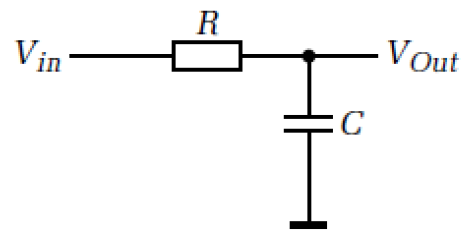
\includegraphics[width=\columnwidth]{images/tiefpass_ordnung_1.png}
\end{minipage}
\hfill
\begin{minipage}[c]{0.45\columnwidth}
    % $$ \text{UTF: } G(s) = \frac{V_{out}}{V_{in}} = \frac{\frac{1}{s \cdot C}}{R + \frac{1}{s \cdot C}} = \frac{1}{1 + s \cdot \underbrace{R \cdot C}_T} $$
    $$ \boxed{ G(s) = \frac{V_{out}}{V_{in}} = \frac{1}{1 + s \cdot \underbrace{R \cdot C}_T} } $$
\end{minipage}
\hfill
\begin{minipage}[c]{0.23\columnwidth}
    $$ \boxed{ f_{3 \, \deci \bel} = \frac{1}{2 \pi \underbrace{R C}_T} } $$
\end{minipage}

\textbf{Hinweis:} Die Zeitkonstante $T$ entspricht immer dem Parameter vor dem $s$. 
Beim Tiefpass 1. Ordnung entspricht dies $T = R \cdot C$

\subsection{Bodeplot Tiefpassfilter 1. und 2. Ordnung}

\begin{minipage}[t]{0.48\columnwidth}
    \begin{center}
        \myul{1. Ordnung}
    \end{center}
    \begin{itemize}
        \item Abfall von $- 20 \deci \bel$ / Dekade
        \item Phasenschiebung von maximal $- 90 \degree$ (bei $f_g = -45 \degree$)
    \end{itemize}
\end{minipage}
\hfill
\begin{minipage}[t]{0.48\columnwidth}
    \begin{center}
        \myul{2. Ordnung}
    \end{center}
    \begin{itemize}
        \item Abfall von $- 40 \deci \bel$ / Dekade
        \item Phasenschiebung von maximal $- 180 \degree$ (bei $f_g = -90 \degree$)
    \end{itemize}
\end{minipage}


\subsection{Filter 2. Ordnung}

\subsubsection{Kaskadierung von zwei gleichen Filtern}

\begin{minipage}[c]{0.48\columnwidth}
    $$ G_{11}(s) = \frac{1}{1 + s \cdot \underbrace{R \cdot C}_{T_2}} \cdot \frac{1}{1 + s \cdot \underbrace{R \cdot C}_{T_2}} $$
\end{minipage}
\hfill
\begin{minipage}[c]{0.48\columnwidth}
    $$ T_2 = \frac{\sqrt{\sqrt{2} - 1}}{2 \pi f_{3 \, \deci \bel} } \approx 0.64 \cdot T_1  $$
\end{minipage}

Daraus folgt, dass bei 2 identischen Stufen die Grenzfrequenz $f_{3 \, \deci \bel}$ der einzelnen Stufen $\frac{1}{0.64} = 1.56$ mal 
\textbf{höher} gewählt werden muss als bei einem Filter 1. Ordnung.


\subsubsection{Filter 2. Ordnung mit komplexen Polen}

\begin{minipage}[c]{0.6\columnwidth}
    $$ G(s) = \frac{A_0 \cdot p_1 \cdot p_2}{(p_1 + s) \cdot (p_2 + s)} = \frac{A_0 \cdot \omega_0^2}{s^2 + \frac{\omega_0}{Q} s + \omega_0^2} $$
$$ p_{1,2} = \frac{\omega_0}{2 Q} (1 \pm \sqrt{1 - 4 Q^2}) $$
\end{minipage}
\hfill
\begin{minipage}[c]{0.38\columnwidth}
    \begin{tabular}{ll}
        $p_i$       & Polstellen \\
                    & komplex für $Q > \frac{1}{2}$ \\
        $Q$         & Polgüte / Filtergüte \\
        $\omega_0$  & Polfrequenz
    \end{tabular}
\end{minipage}



% bei Platzmangel weglassen
\subsection{Filter höherer Ordnung}

\begin{itemize}
    \item Systeme höherer Ordnung können aufgeteilt werden in kaskadierte Teilsysteme 1. und 2. Ordnung
    \item Höhere Ordnung und komplexe Pole ermöglichen steileren Übergang zwischen Durchlass- und Sperrbereich
\end{itemize}

Folgende Filter erzielen durch unterschiedliche Polverteilungen unterschiedliches Verhalten:

\begin{itemize}
    \item \textbf{Butterworth:} Konstant im Durchlassbereich der UTF
    \item \textbf{Bessel:} Beste Rechteckübertragung, kein Überschwingen
    \item \textbf{Tschebyscheff:} Steilster Abfall im Sperrbereich der UTF
\end{itemize}


\subsection{Zeitverhalten: Schrittantwort}

\begin{enumerate}
    \item Frenqenzbereich: \textbf{Multiplikation} der UTF mit $\frac{1}{s}$
    \item Rücktransformation in den Zeitbereich, um $t_{step}(t)$ zu erhalten
\end{enumerate}


\subsubsection{Tiefpass 1. Ordnung}

\begin{minipage}[c]{0.48\columnwidth}
    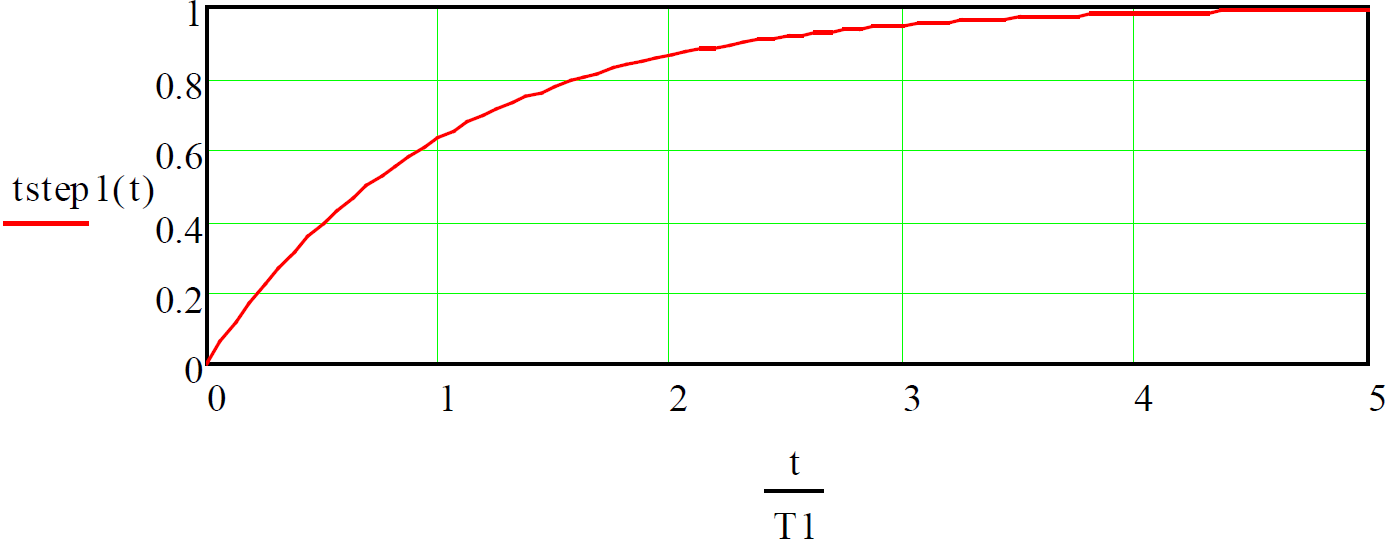
\includegraphics[width=\columnwidth]{images/schrittantwort_tp_ordnung_1.png}
\end{minipage}
\hfill
\begin{minipage}[c]{0.48\columnwidth}
    $$  t_{step,1}(t) = 1 - e^{- \frac{t}{T_1}} $$
\end{minipage}


\subsubsection{Tiefpass 2. Ordnung}

\begin{minipage}[c]{0.43\columnwidth}
    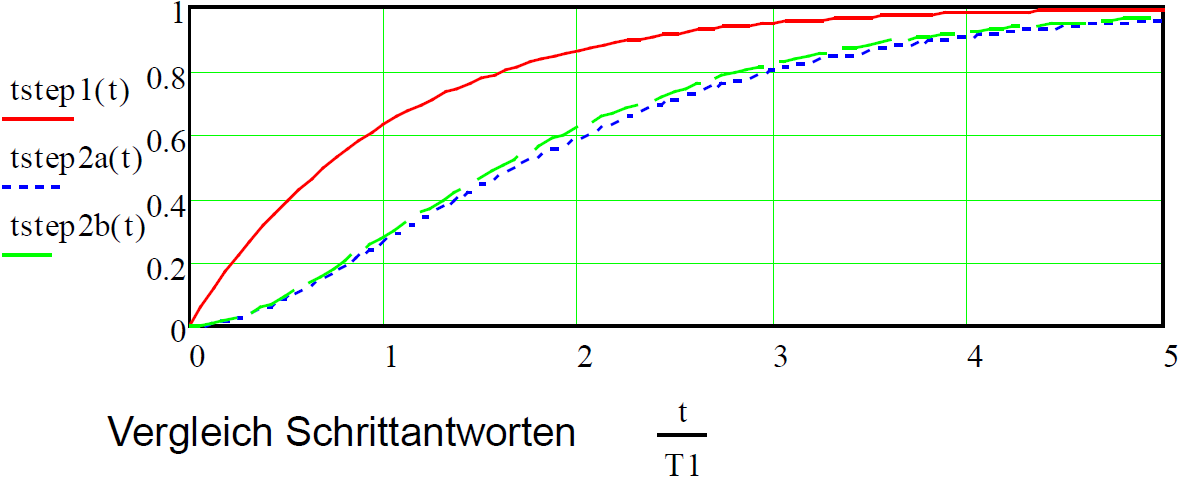
\includegraphics[width=\columnwidth]{images/schrittantworten_vergleich.png}
\end{minipage}
\hfill
\begin{minipage}[c]{0.55\columnwidth}
    $$ t_{step2a}(t) = 1 - e^{- \frac{t}{T_1}}\cdot \Big( 1 + \frac{t}{T_1} \Big) $$
    $$ t_{step2b}(t) = 1 - \Big( \frac{T_1 \cdot e^{- \frac{t}{T_1}} - T_2 \cdot e^{- \frac{t}{T_2}}}{T_1 - T_2} \Big) $$
\end{minipage}


\subsection{Schrittantworten verschiedener Polgüten}

\begin{minipage}[c]{0.48\columnwidth}
    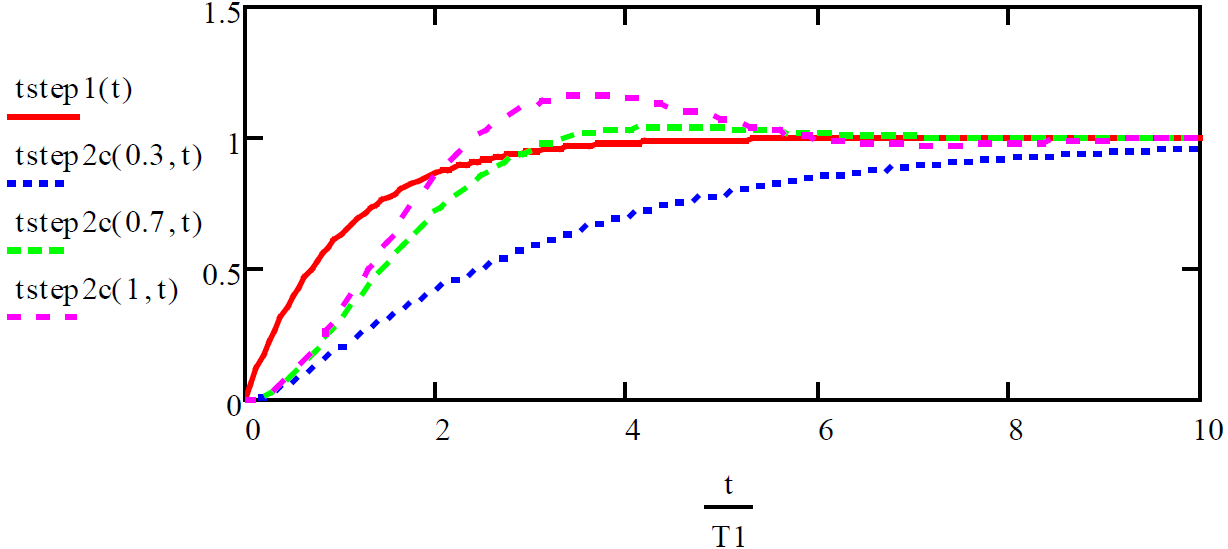
\includegraphics[width=\columnwidth]{images/schrittantwort_verschiedene_polgueten.png}
\end{minipage}
\hfill
\begin{minipage}[c]{0.48\columnwidth}
    Komplexe Pole ($Q > 0$) führt zu Überschwingern. \\
    Bei einer Polgüte von $Q = \frac{1}{\sqrt{2}} \approx 0.7$ (\cgn{grüne Kruve}) schwingt das System am schnellsten ein!
\end{minipage}


\subsection{Filter 2. Ordnung}

\begin{minipage}[c]{0.48\columnwidth}
    \begin{center}
        \myul{\textbf{Tiefpass}}
    \end{center}
    $$ \boxed{ G(s) = \frac{V_{out}}{V_{in}} = \frac{A_0}{1 + \frac{1}{\omega_0 \cdot Q} s + \frac{1}{\omega_0^2} s^2 } } $$
\end{minipage}
\hfill
\begin{minipage}[c]{0.48\columnwidth}
    \begin{center}
        \myul{\textbf{Bandpass}}
    \end{center}
    % CHECK gilt das für aktive und / order passive Filter?
    $$ \boxed{ G(s) = \frac{V_{out}}{V_{in}} = \frac{A \cdot \frac{\omega_0}{Q} \cdot s}{s^2 +  \frac{\omega_0}{Q} s + \omega_0^2 } } $$
\end{minipage}

Passive RC-Filter können maximal Güte $0.5$ haben (entkoppelte reelle Pole). Filter höherer Güte benötigen entweder
Spulen oder \textbf{Verstärker}.


\example{UTF Tiefpass 2. Ordnung}

\begin{minipage}[c]{0.4\columnwidth}
    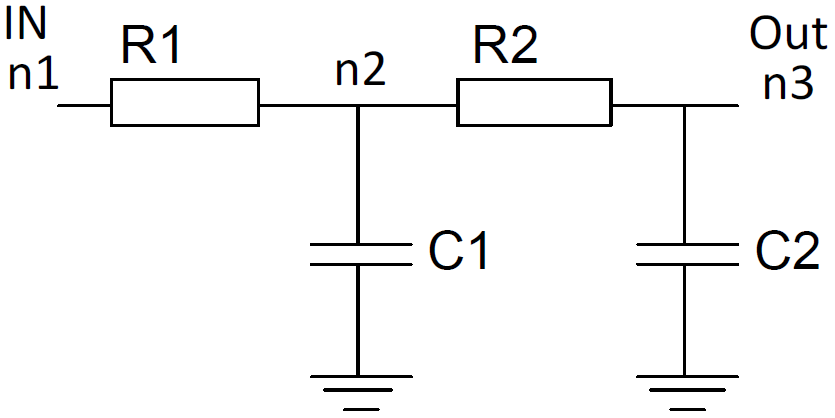
\includegraphics[width=\columnwidth]{images/tiefpass_ordnung_2.png}
\end{minipage}
\hfill
\begin{minipage}[c]{0.58\columnwidth}
    $$ A_0 = 1 \qquad \omega_0 = \frac{1}{\sqrt{C_1 C_2 R_1 R_2}} $$
    $$ Q = \frac{\sqrt{C_1 C_2 R_1 R_2}}{C_1 R_1 + C_2 R_1 + C_2 R_2} $$
\end{minipage}
$$ G(s) = \frac{V_{out}}{V_{in}} = \frac{1}{1 + (C_1 R_1 + C_2 R_1 + C_2 R_2) \cdot s + C_1 C_2 R_1 R_2 \cdot s^2 } $$


% --------------------------------------------------------------------------------------------------------------------------
% \section{Aktive Filter} 

\subsection{Sallen-Key-Filter (Einfachmitkopplung)}

\begin{minipage}[c]{0.4\columnwidth}
    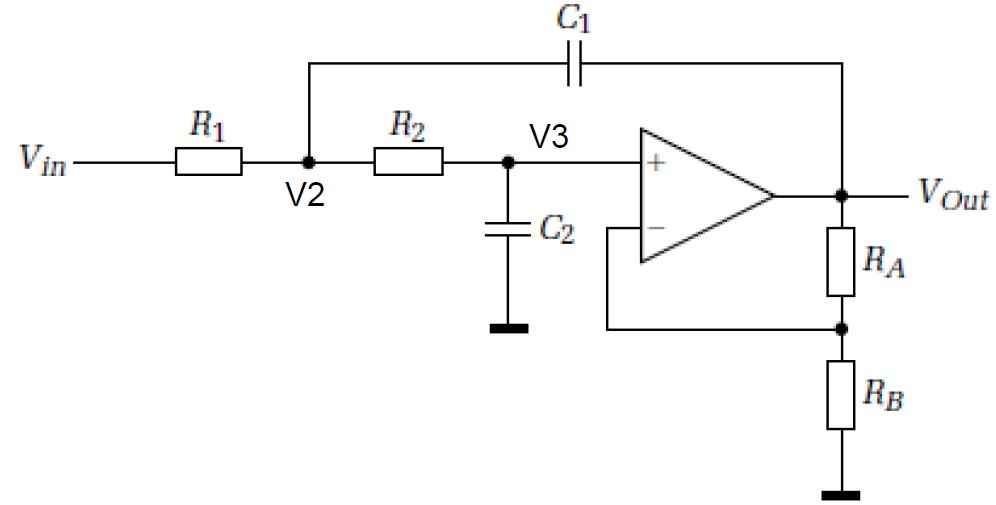
\includegraphics[width=\columnwidth]{images/sallen_key.png}
\end{minipage}
\hfill
\begin{minipage}[c]{0.58\columnwidth}
    $$ \text{OpAmp:} \quad  V_{out} = G_0 \cdot V_3 = \Big(1 + \frac{R_A}{R_B} \Big) \cdot V_3 $$
    $$ \omega_0 = \frac{1}{\sqrt{C_1 C_2 R_1 R_2}} $$
    $$ Q = \frac{\sqrt{C_1 C_2 R_1 R_2}}{ C_2 (R_1 + R_2) + C_1 R_1 \cdot (1 - G_0)} $$
\end{minipage}

$$ \boxed{ G(s) = \frac{G_0}{ C_1 C_2 R_1 R_2 \cdot s^2 + [ C_2 (R_1 + R_2) + C_1 R_1 (1 - G_0) ] \cdot s + 1} } $$

\textbf{Stromgleichungen:}
\begin{align*}
    \text{V2:} \quad 0 &= (V_2 - V_{in}) \frac{1}{R_1} + (V_2 - V_3) \frac{1}{R_2} + (V_2 - V_{out}) \cdot s \cdot C_1  \\
    \text{V3:} \quad 0 &= (V_3 - V_2) \frac{1}{R_2} + V_3  \cdot s \cdot C_2 
\end{align*}


\subsubsection{Sallen-Key-Filter bei hohen Frequnezen}

\begin{minipage}[c]{0.4\columnwidth}  
    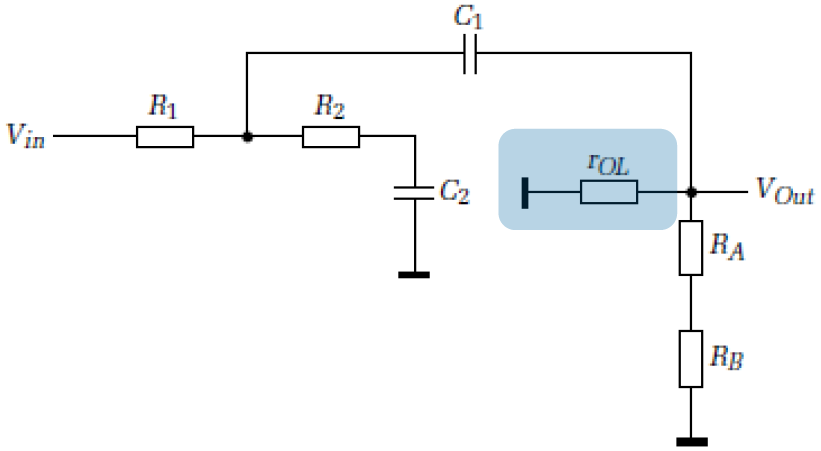
\includegraphics[width=\columnwidth]{images/sallen_key_hohe_frequenzen.png}
\end{minipage}
\hfill
\begin{minipage}[c]{0.58\columnwidth}
    $$ \boxed{ \frac{V_{out}}{V_{in}} = \approx \frac{r_{OL}}{R_1 + r_{OL}} }$$
    $r_{OL}$ ist der OpAmp open-loop Ausgangswiderstand (bei hohen Frequenzen $\approx 100 \, \ohm$)
\end{minipage}

\begin{itemize}
    \item Dämpfung ist limitiert auf obigen Spannungsteiler
        \textrightarrow\ Sallen-Key-Filter sind nicht geeignet für Systeme mit hohen Frequenzanteilen z.B. PWM-DAC
\end{itemize}


\subsection{Multiple-Feedback-Struktur}

\begin{minipage}[c]{0.4\columnwidth}
    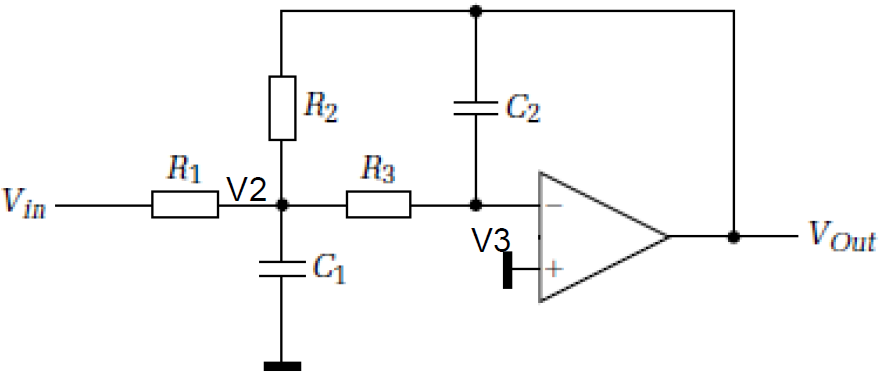
\includegraphics[width=\columnwidth]{images/aktive_filter_multiple_feedback.png}
\end{minipage}
\hfill
\begin{minipage}[c]{0.58\columnwidth}
    $$ \text{OpAmp:} \quad  G_0 = -\frac{R_2}{R_1} $$
    $$ Q = \frac{\sqrt{C_1 C_2 R_1 R_2}}{ C_2 \Big( R_2 + R_2 + R_3 \frac{R_2}{R_1} \Big)} $$
\end{minipage}

$$ \boxed{ G(s) = \frac{G_0}{1 + C_2 \Big( R_2 + R_2 + R_3 \frac{R_2}{R_1} \Big) \cdot s + C_1 C_2 R_2 R_3 \cdot s^2 }}$$

\textbf{Stromgleichungen:}
\begin{align*}
    \text{V2:} \quad 0 &= (V_2 - V_{in}) \frac{1}{R_1} + (V_2 - V_{out}) \frac{1}{R_2} + (V_2 - V_3) \frac{1}{R_3} + V_2 \cdot s \cdot C_1  \\
    \text{V3:} \quad 0 &= (V_3 - V_2) \frac{1}{R_3} + (V_3 - V_{out})  \cdot s \cdot C_2 
\end{align*}

\subsection{Sallen-Key vs. Multiple-Feedback Struktur}

\begin{minipage}[t]{0.48\columnwidth}
    \begin{center}
        \myul{\textbf{Sallen-Key}}
    \end{center}
    \begin{outline}
        \1 Nicht-invertierend
        \1 $Q$ sensitiver auf Toleranzen
        \1 Vorwärtspfad für hohe Frequenzen
        \1 Noise-Gain: $A$
        \1 Eher für 
            \2 Hochpass
            \2 kleine Verstärkungen
    \end{outline}
\end{minipage}
\hfill
\begin{minipage}[t]{0.48\columnwidth}
    \begin{center}
        \myul{\textbf{Multiple-Feedback}}
    \end{center}
    \begin{outline}
        \1 Invertierend
        \1 $f_g$ sensitiver auf Toleranzen 
        \\
        \1 Noise-Gain: $A+1$
        \1 Eher für 
            \2 Tiefpass, Bandpass
            \2 grössere Verstärkungen
    \end{outline}
\end{minipage}


% CHECK Wohin mit dieser subsection?
\subsection{Vorgehen: UTF aus OPV-Filterschaltung ermitteln}
\begin{itemize}
    \item Stromgleichungen (Knotengleichungen) aufstellen
    \item Gleichungen ineinander einsetzen
    \item Umformen nach $G(s) = \frac{V_{out}}{V_{in}}$
\end{itemize}


% ---------------------------------------------------------------------------------------------------------------------
% \section{Zustandsvariablen-Filter (Biquad-Filter)}

\subsection{Zustandsvariablen-Filter (Biquad-Filter)}
\label{zustandsvariablenfilter}

\begin{minipage}[c]{0.6\columnwidth}
    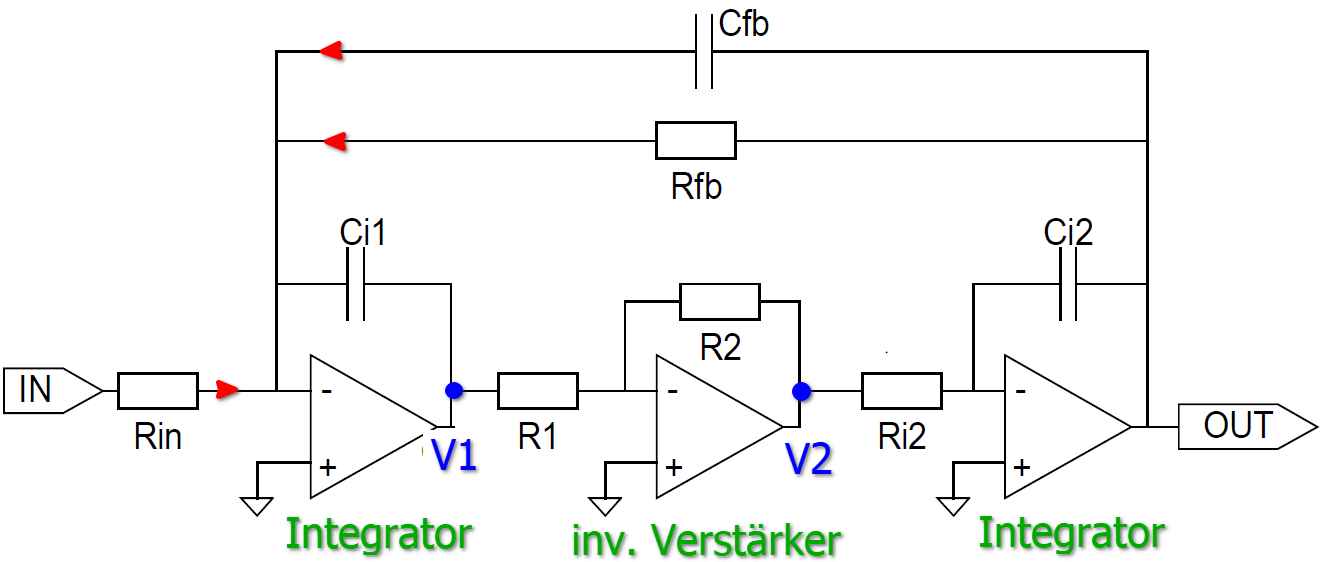
\includegraphics[width=\columnwidth]{images/zustandsvariablenfilter.png}
\end{minipage}
\hfill
\begin{minipage}[c]{0.38\columnwidth}
    Mit dieser Topologie sind alle drei \textbf{Parameter} $f_0$, $Q$ und $A_0$ \textbf{frei wählbar!} \\
    An $V_{out}$ herrscht \textbf{Tiefpass-Verhalten.}
\end{minipage}

$$ \boxed{ G(s) = \frac{- \frac{R_{fb}}{R_{in}}}{s^2 \cdot C_{i1} C_{i2} R_{fb} R_{i2} \frac{R_1}{R_2} + s \cdot C_{fb} R_{fb} + 1} } $$

$$ f_0 = \frac{1}{2 \pi \sqrt{C_{i1} C_{i2} R_{fb} R_{i2} \frac{R_1}{R_2}}} \qquad Q = \frac{1}{C_{fb}} \sqrt{C_{i1} C_{i2} \frac{R_1}{R_2 R_{fb}} } 
\qquad A_0 = - \frac{R_{fb}}{R_{in}} $$


\subsubsection{Allgemein: FIlter mit mehreren OpAmps}

Mit der Filter-Struktur aus Abschnitt ~\ref{zustandsvariablenfilter} können auch Bandpass- und Hochpass-Filter gebildet werden:
\begin{itemize}
    \item \textbf{Tiefpass:} Abgriff beim 3. OpAmp ($V_{out}$ gemäss Abschnitt ~\ref{zustandsvariablenfilter})
    \item \textbf{Bandpass:} Abgriff beim 2. OpAmp (an Knoten V2)
    \item \textbf{Hochpass:} Abgriff beim 2. OpAmp, Einspeisung am neg. Eingang des 2. OpAmps 
\end{itemize}


% -----------------------------------------------------------------------------------------------------------------------   
% \section{Analyse von Filterschaltungen mit Signalflussdiagrammen}
\subsection{Analyse von Filterschaltungen mit Signalflussdiagrammen}

Aktive Filterschaltungen (mit OpAmps) können mittels Signalflussdiagrammen (SFDs) analysiert werden. Dazu wird die gesamte Schaltung
in einzelne Komponenten aufgeteilt. Diese Komponeten werden dann mit Impedanz- bzw. Admittanzfunktionen abgebildet.
Um die Übertragungsfunktion (UTF) der gesamten Schaltung zu erhalten, muss die \textbf{Regel von Mason} angewendet werden.

% TODO: formatting..? -> gseht scheisse us
\subsubsection{Eingangsadmittanzen / (Eingangsimpedanzen)}

\textbf{Hinweis:} Es wird normalerweise mit Eingangs\textbf{admittanzen} gearbeitet!

\begin{tabular}{lll}
    \textbf{Komponente} & \textbf{Admittanz} $\bm{Y}$       & (\textbf{Impedanz} $\bm{Z}$) \\
    \midrule
    Widerstand $R$      & $Y_{res} = \frac{1}{R}$           & ($Z_{res} = R$  )\\
    Kapazität $C$       & $Y_{cap} = s \cdot C$             & ($Z_{cap} = \frac{1}{s \cdot C}$)\\
    Induktivität $L$    & $Y_{ind} = \frac{1}{s \cdot L}$   & ($Z_{ind} = s \cdot L$)
\end{tabular}


% TODO: formatting..? -> gseht scheisse us
\subsubsection{OpAmp Impedanzfunktionen}

\textbf{Hinweis:} Es geht um \textbf{negatives Feedback} bzw. \textbf{Gegenkopplung}

\begin{tabular}{ll}
    \textbf{Schaltung (Feedback)}       & \textbf{Impedanz} $\bm{Z}$ \\
    \midrule
    Widerstand $R_f$ im Feedback        & $Z_{op} = - R_f$ \\
    Kapazität $C_f$ im Feedback         & $Z_{op} = - \frac{1}{s \cdot C_f}$ \\
    $R_f C_f$ (parallel) im Feedback    & $Z_{op} = - \frac{R_f}{1 + s \cdot C_f \cdot R_f}$
\end{tabular}


\example{Summierender Verstärker}

\begin{minipage}[c]{0.4\columnwidth}
    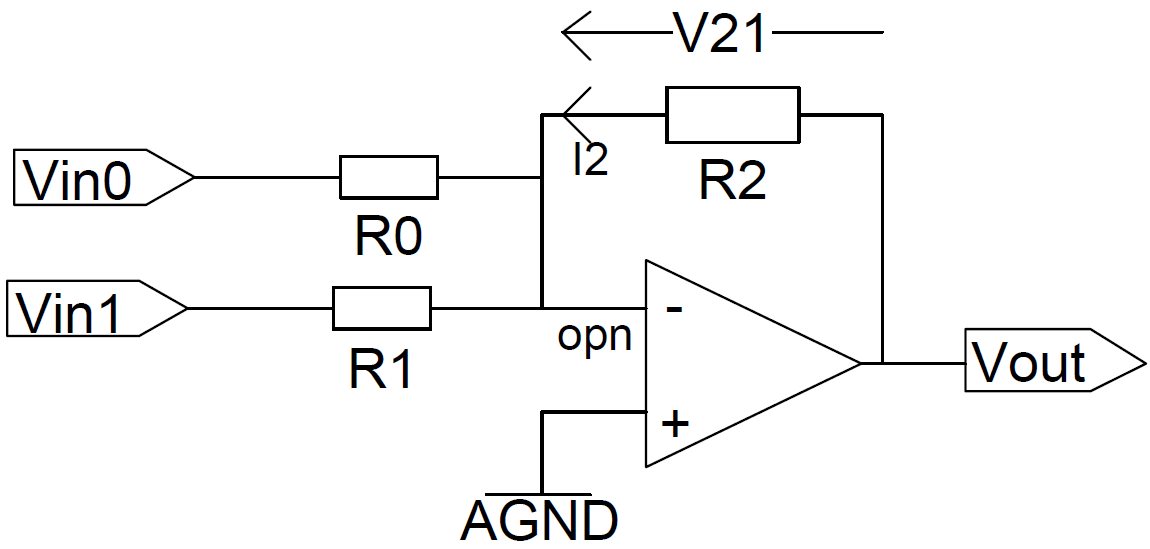
\includegraphics[width=\columnwidth]{images/summierender_verstaerker.png}
\end{minipage}
\hfill
\begin{minipage}[c]{0.58\columnwidth}
    \begin{center}
        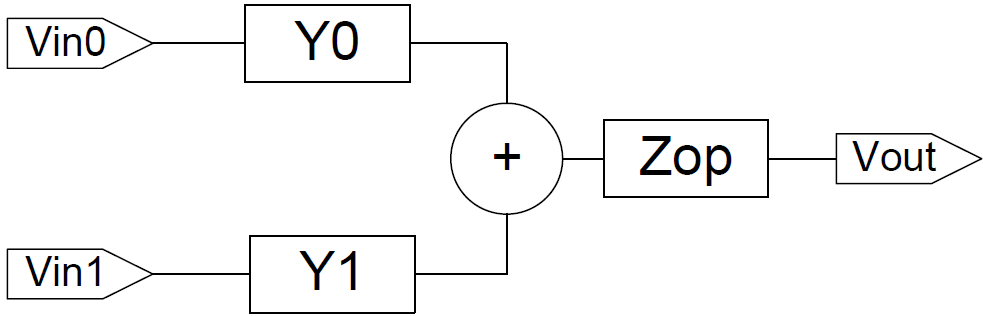
\includegraphics[width=0.8\columnwidth]{images/summierender_verstaerker_sfd.png}
    \end{center}
    $$ V_{out} = Z_{op} \cdot (Y_0 \cdot V_{in0} + Y_1 \cdot V_{in1}) $$
\end{minipage}

$$ Y_0 = \frac{1}{R_0} \qquad Y_1 = \frac{1}{R_1} \qquad Z_{op} = - R_f $$


\example{Aktiver Tiefpass 1. Ordnung}

\begin{minipage}[c]{0.4\columnwidth}
    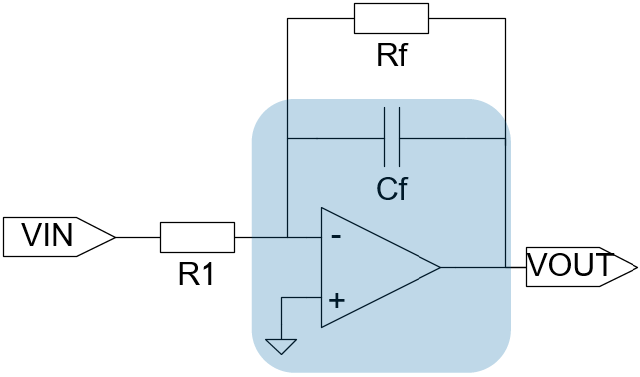
\includegraphics[width=\columnwidth]{images/filter_signalflussdiagramme_tiefpass_ordnung_1.png}
\end{minipage}
\hfill
\begin{minipage}[c]{0.48\columnwidth}
    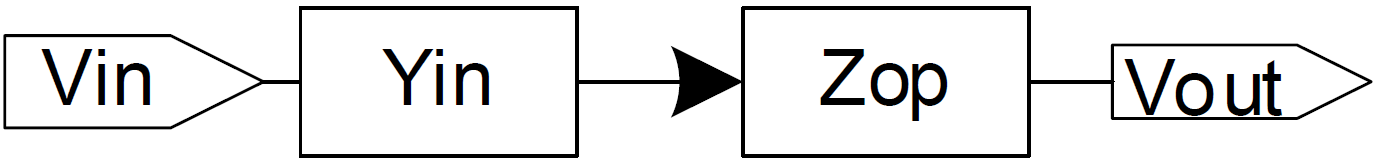
\includegraphics[width=\columnwidth]{images/filter_signalflussdiagramme_tiefpass_ordnung_1_sfd.png}
    $$ Y_{in} = \frac{1}{R_1} \qquad Z_{op} = - \frac{R_f}{1 + s \cdot C_f \cdot R_f} $$
\end{minipage}

$$ G(s)= \frac{V_{out}}{V_{in}} = Y_{in} \cdot Z_{op} =- \frac{R_f}{1 + s \cdot C_f \cdot R_f} \cdot \frac{1}{R_1} $$


\subsection{Allgemein einsezbare Biquads (Zustandsvariablenfilter)}

\subsection{Regel von Mason (vereinfacht)}

$$ \text{UTF:} \quad G(s) = \frac{V_{out}}{V_{in}} = \frac{\text{Produkt der Transmittanzen im Vorwärtspfad}}{1 - \text{Summe aller Schleifentransmittanzen}} $$


\example{Analyse Bandpass mittels SFD und Regel von Mason}

\begin{minipage}[c]{0.48\columnwidth}
    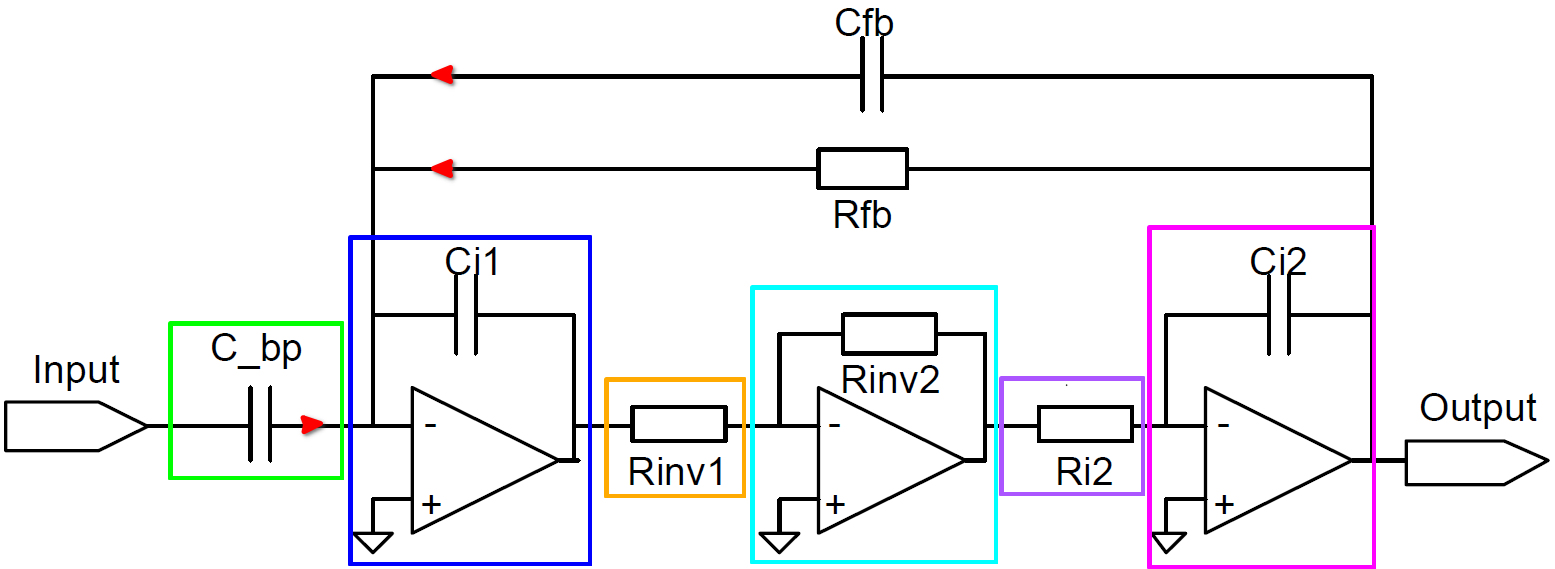
\includegraphics[width=\columnwidth]{images/signalflussdiagramme_bandpass_schaltung.png}
\end{minipage}
\hfill
\begin{minipage}[c]{0.48\columnwidth}
    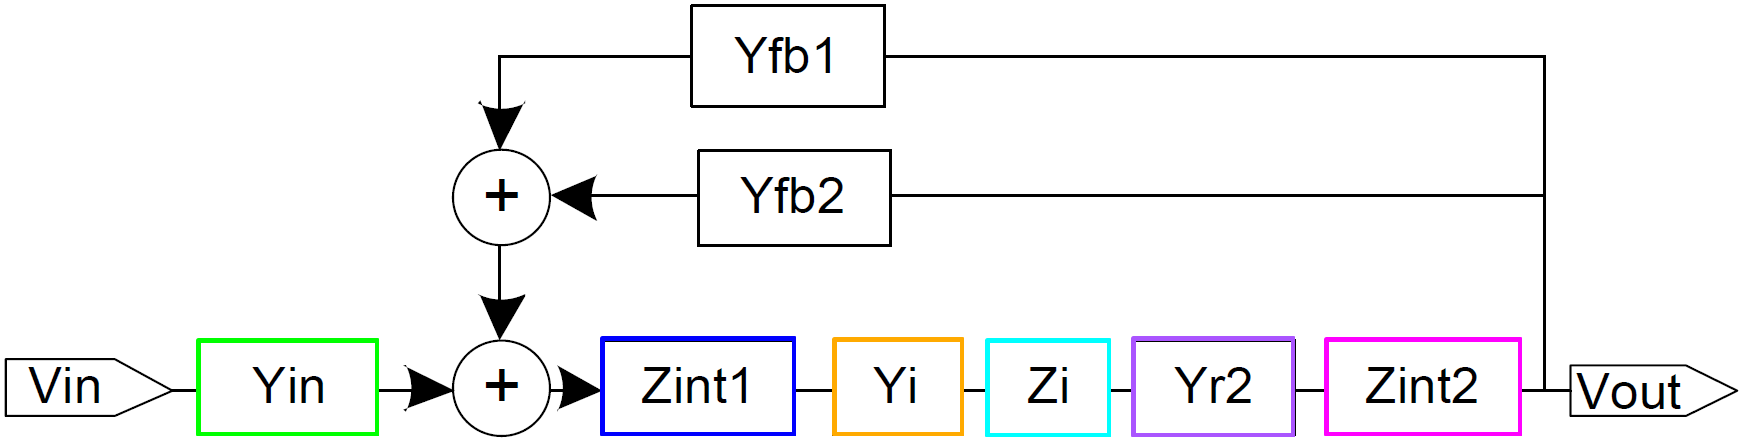
\includegraphics[width=\columnwidth]{images/signalflussdiagramme_bandpass_blockschaltbild.png}
\end{minipage}

$$ G(s) = \frac{V_{out}}{V_{in}} = \frac{Y_{in} \cdot Z_{int1} \cdot Y_i \cdot Z_i \cdot Y_{r2} \cdot Z_{int2} }
    {1 - (Y_{fb1} - Y_{fb2}) \cdot Z_{int1} \cdot Y_i \cdot Z_i \cdot Y_{r2} \cdot Z_{int2} } $$